% A LaTeX template for EXECUTIVE SUMMARY of the MSc Thesis submissions to
% Politecnico di Milano (PoliMi) - School of Industrial and Information Engineering
%
% P. F. Antonietti, S. Bonetti, A. Gruttadauria, G. Mescolini, A. Zingaro
% e-mail: template-tesi-ingind@polimi.it
%
% Last Revision: October 2021
%
% Copyright 2021 Politecnico di Milano, Italy. Inc. All rights reserved.

\documentclass[11pt,a4paper]{article}

%------------------------------------------------------------------------------
%	REQUIRED PACKAGES AND  CONFIGURATIONS
%------------------------------------------------------------------------------
% PACKAGES FOR TITLES
\usepackage{titlesec}
\usepackage{color}

% PACKAGES FOR LANGUAGE AND FONT
\usepackage[utf8]{inputenc}
\usepackage[english]{babel}
\usepackage[T1]{fontenc} % Font encoding
% PACKAGES FOR IMAGES
\usepackage{graphicx}
\graphicspath{{Images/}} % Path for images' folder
\usepackage{eso-pic} % For the background picture on the title page
\usepackage{subfig} % Numbered and caption subfigures using \subfloat
\usepackage{caption} % Coloured captions
\usepackage{transparent}

% STANDARD MATH PACKAGES
\usepackage{amsmath}
\usepackage{amsthm}
\usepackage{bm}
\usepackage[overload]{empheq}  % For braced-style systems of equations

% PACKAGES FOR TABLES
\usepackage{tabularx}
\usepackage{longtable} % tables that can span several pages
\usepackage{colortbl}

% PACKAGES FOR ALGORITHMS (PSEUDO-CODE)
\usepackage{algorithm}
\usepackage{algorithmic}

% PACKAGES FOR REFERENCES & BIBLIOGRAPHY
\usepackage[colorlinks=true,linkcolor=black,anchorcolor=black,citecolor=black,filecolor=black,menucolor=black,runcolor=black,urlcolor=black]{hyperref} % Adds clickable links at references
\usepackage{cleveref}
\usepackage[square, numbers, sort&compress]{natbib} % Square brackets, citing references with numbers, citations sorted by appearance in the text and compressed
\bibliographystyle{plain} % You may use a different style adapted to your field

% PACKAGES FOR THE APPENDIX
\usepackage{appendix}

% PACKAGES FOR ITEMIZE & ENUMERATES
\usepackage{enumitem}

% OTHER PACKAGES
\usepackage{amsthm,thmtools,xcolor} % Coloured "Theorem"
\usepackage{comment} % Comment part of code
\usepackage{fancyhdr} % Fancy headers and footers
\usepackage{lipsum} % Insert dummy text
\usepackage{tcolorbox} % Create coloured boxes (e.g. the one for the key-words)
\usepackage{stfloats} % Correct position of the tables
\usepackage{multirow}
\usepackage{multicol}





%-------------------------------------------------------------------------
%	NEW COMMANDS DEFINED
%-------------------------------------------------------------------------
% EXAMPLES OF NEW COMMANDS -> here you see how to define new commands
\newcommand{\bea}{\begin{eqnarray}} % Shortcut for equation arrays
\newcommand{\eea}{\end{eqnarray}}
\newcommand{\e}[1]{\times 10^{#1}}  % Powers of 10 notation
\newcommand{\mathbbm}[1]{\text{\usefont{U}{bbm}{m}{n}#1}} % From mathbbm.sty
\newcommand{\pdev}[2]{\frac{\partial#1}{\partial#2}}
% NB: you can also override some existing commands with the keyword \renewcommand

%----------------------------------------------------------------------------
%	ADD YOUR PACKAGES (be careful of package interaction)
%----------------------------------------------------------------------------
\usepackage{amsfonts} 
\usepackage[font=footnotesize,labelfont=bf]{caption}

%----------------------------------------------------------------------------
%	ADD YOUR DEFINITIONS AND COMMANDS (be careful of existing commands)
%----------------------------------------------------------------------------
\usepackage{import}
\usepackage{xifthen}
\usepackage{pdfpages}
\usepackage{transparent}
\usepackage{wrapfig}
\usepackage{dsfont}
\usepackage{shadethm}
\usepackage{tikz}
\usepackage{pgfplots}


\parindent=0pt

\newcommand{\incfig}[1]{%
    \def\svgwidth{\columnwidth}
    \import{./Images/}{#1.pdf_tex}
}
\newcommand{\real}{\mathbb{R}}
\newcommand*{\oldepsilon}{\epsilon}
\renewcommand*{\epsilon}{\varepsilon}
\DeclareMathOperator*{\esssup}{ess\,sup}
\DeclareMathOperator*{\essinf}{ess\,inf}

\newcommand{\oldphi}{\phi}
\renewcommand{\phi}{\varphi}

\newcommand{\oldrho}{\rho}
\renewcommand{\rho}{\varrho}



\numberwithin{equation}{section}
%----------------------------------------------------------------------------
%	CONFIGURATION OF THEOREM ENVIRONMENTS


% \newtheoremstyle{break}
%     {\partopsep}{\topsep}%  
%     {\normalfont}{}
%     {\bfseries}{}%
%     {\newline}{}%
% \theoremstyle{break}
% \newtheorem{theorem}{Theorem}[section]
% \newtheorem{corollary}{Corollary}[section]
% \newtheorem{proposition}{Proposition}[section]
% \newtheorem{remark}{Remark}[section]
% \newtheorem{lemma}{Lemma}[section]
% \newtheorem{notation}{Notation}[section]
% \newtheorem{definition}{Definition}[section]

% \newtheorem{definition}{Definition}[section]

% \newtheorem*{remark}{Remark}

% \newtheorem{lemma}{Lemma}[section]
% %----------------------------------------------------------------------------

% Do not change Configuration_files/config.tex file unless you really know what you are doing.
% This file ends the configuration procedures (e.g. customizing commands, definition of new commands)
% Set the geometric layout of the document
\usepackage{geometry}
\geometry{
  top=3cm,
  left = 2.0cm,
  right = 2.0cm,
  bottom=2cm,
  headheight= 2cm,
  headsep= 0cm,
}
\raggedbottom

% Create color bluePoli (-> manuale grafica coordinata:  https://www.polimi.it/fileadmin/user_upload/il_Politecnico/grafica-coordinata/2015_05_11_46xy_manuale_grafica_coordinata.pdf)
\definecolor{bluePoli}{cmyk}{0.4,0.1,0,0.4}

% Custom theorem environments
\declaretheoremstyle[
  shaded={rulecolor=bluePoli!20, rulewidth=1pt, bgcolor=bluePoli!5},
  headfont=\color{bluePoli}\normalfont\bfseries,
  bodyfont=\color{black}\normalfont,
]{colored}

\captionsetup[figure]{labelfont={color=bluePoli}} % Set colour of the captions
\captionsetup[table]{labelfont={color=bluePoli}} % Set colour of the captions
\captionsetup[algorithm]{labelfont={color=bluePoli}} % Set colour of the captions

\theoremstyle{colored}
\newtheorem{theorem}{Theorem}[section]
\newtheorem{proposition}{Proposition}[section]
\newtheorem{definition}{Definition}[section]
\newtheorem*{remark}{Remark}
\newtheorem{lemma}{Lemma}[section]

% Enhances the features of the standard "table" and "tabular" environments.
\newcommand\T{\rule{0pt}{2.6ex}}
\newcommand\B{\rule[-1.2ex]{0pt}{0pt}}

% Algorithm description
\newcounter{algsubstate}
\renewcommand{\thealgsubstate}{\alph{algsubstate}}
\newenvironment{algsubstates}{
    \setcounter{algsubstate}{0}%
    \renewcommand{\STATE}{%
    \stepcounter{algsubstate}%
    \Statex {\small\thealgsubstate:}\space}
    }{}

% Custom theorem environment
\newcolumntype{L}[1]{>{\raggedright\let\newline\\\arraybackslash\hspace{0pt}}m{#1}}
\newcolumntype{C}[1]{>{\centering\let\newline\\\arraybackslash\hspace{0pt}}m{#1}}
\newcolumntype{R}[1]{>{\raggedleft\let\newline\\\arraybackslash\hspace{0pt}}m{#1}}

% Custom itemize environment
\setlist[itemize,1]{label=$\bullet$}
\setlist[itemize,2]{label=$\circ$}
\setlist[itemize,3]{label=$-$}
\setlist{nosep}

% Set separation of columns
\setlength{\columnsep}{30pt}

% Create command for background pic
\newcommand\BackgroundPic{% Adding background picture
	\put(230,358){
		\parbox[b][\paperheight]{\paperwidth}{%
			\vfill
			\centering
			\transparent{0.2}
			
\includegraphics[width=0.8\paperwidth]{raggiera_polimi.eps}%
			\vfill
}}}

% Set indentation
%\setlength\parindent{0pt}

% Custom title commands
\titleformat{\section}
{\color{bluePoli}\normalfont\Large\bfseries}
{\color{bluePoli}\thesection.}{1em}{}
\titlespacing*{\section}
{0pt}{2ex}{1ex}

\titleformat{\subsection}
{\color{bluePoli}\normalfont\large\bfseries}
{\color{bluePoli}\thesubsection.}{1em}{}
\titlespacing*{\subsection}
{0pt}{2ex}{1ex}

\titleformat{\subsubsection}
{\color{bluePoli}\normalfont\normalsize\bfseries}
{\color{bluePoli}\thesubsubsection.}{1em}{}
\titlespacing*{\subsubsection}
{0pt}{2ex}{1ex}

% Custom headers and footers
\pagestyle{fancy}
\fancyhf{}

\fancyfoot{}
\fancyfoot[C]{\thepage} % page
\renewcommand{\headrulewidth}{0mm} % headrule width
\renewcommand{\footrulewidth}{0mm} % footrule width

\makeatletter
\patchcmd{\headrule}{\hrule}{\color{black}\hrule}{}{} % headrule
\patchcmd{\footrule}{\hrule}{\color{black}\hrule}{}{} % footrule
\makeatother

% -> Create the header
\chead[C]{
\centering
\begin{tcolorbox}[arc=0pt, boxrule=0pt, colback=bluePoli!60, width=\textwidth, colupper=white]
    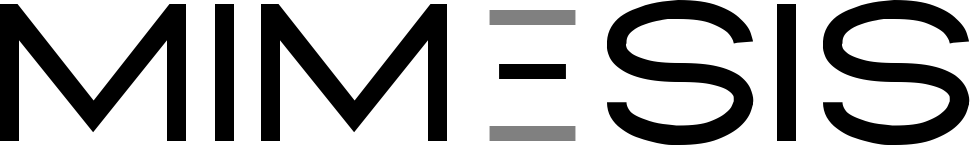
\includegraphics[width=0.2\textwidth]{mimesis.png}
\end{tcolorbox}
}


% Insert here the info that will be displayed into your Title page
% -> title of your work
\renewcommand{\title}{\noindent The KPP-Fisher equation over simple graphs} 

% -> author name and surname
\renewcommand{\author}{Andrea Bonifacio}
% -> MSc course
\newcommand\norm[1]{\lVert#1\rVert}
\newcommand{\course}{Reaction Diffusion Equations}
% -> advisor name and surname
\newcommand{\advisor}{Gianmaria Verzini}
% IF AND ONLY IF you need to modify the co-supervisors you also have to modify the file Configuration_files/title_page.tex (ONLY where it is marked)
%\newcommand{\firstcoadvisor}{Name Surname} % insert if any otherwise comment
%\newcommand{\secondcoadvisor}{Name Surname} % insert if any otherwise comment
% -> academic year
\newcommand{\YEAR}{2023-2024}

%-------------------------------------------------------------------------
%	BEGIN OF YOUR DOCUMENT
%-------------------------------------------------------------------------
\begin{document}
%-----------------------------------------------------------------------------
% TITLE PAGE
%-----------------------------------------------------------------------------
% Do not change Configuration_files/TitlePage.tex (Modify it IF AND ONLY IF you need to add or delete the Co-advisors)
% This file creates the Title Page of the document
% DO NOT REMOVE SPACES BETWEEN LINES!

%\twocolumn[{\begin{@twocolumnfalse}

\AddToShipoutPicture*{\BackgroundPic}

\hspace{-0.6cm}
\includegraphics[width=0.6\textwidth]{logo_polimi_ing_indinf.eps}

\vspace{-1mm}
\fontsize{0.3cm}{0.5cm}\selectfont \bfseries \textsc{\color{bluePoli} Report}\\

\vspace{-0.2cm}
\Large{\textbf{\color{bluePoli}{\title}}}\\

\vspace{-0.2cm}
\fontsize{0.3cm}{0.5cm}\selectfont \bfseries \textsc{\color{bluePoli} \course}\\

\vspace{-0.2cm}
\fontsize{0.3cm}{0.5cm} \selectfont \bfseries Authors: \textsc{\textbf{\author}}\\

%\vspace{-0.4cm}
%\fontsize{0.3cm}{0.5cm}\selectfont \bfseries Advisor: \textsc{\textbf{\advisor}}\\

% if only ONE co-advisor is present:
%\vspace{-0.4cm}
%\fontsize{0.3cm}{0.5cm}\selectfont \bfseries Co-advisor: \textsc{\textbf{\firstcoadvisor}}\\
% if more than one co-advisors are present:
%\vspace{-0.4cm}
%\fontsize{0.3cm}{0.5cm}\selectfont \bfseries Co-advisors: \textsc{\textbf{\firstcoadvisor}}\textsc{\textbf{\secondcoadvisor}}\\

\vspace{-0.4cm}
\fontsize{0.3cm}{0.5cm}\selectfont \bfseries Academic year: \textsc{\textbf{\YEAR}}

\small \normalfont

\vspace{11pt}

\centerline{\rule{1.0\textwidth}{0.4pt}}

%\vspace{15pt}
%\end{@twocolumnfalse}}]

\thispagestyle{plain} % In order to not show the header in the first page


%%%%%%%%%%%%%%%%%%%%%%%%%%%%%%
%%     THESIS MAIN TEXT     %%
%%%%%%%%%%%%%%%%%%%%%%%%%%%%%%


%-----------------------------------------------------------------------------
% INTRODUCTION
%-----------------------------------------------------------------------------

\section{Introduction}

Numerical simulations play a critical role in a wide array of scientific and engineering applications, providing insights into the behavior of physical systems under various conditions. Among the most prominent techniques for performing such simulations is Finite Element Modeling (FEM). FEM discretizes a continuous domain into a mesh of finite elements, allowing for the approximation of solutions to complex partial differential equations (PDEs). However, one significant drawback of FEM is its computational intensity, especially when high resolution is required for accurate results. This research aims to explore the potential of Deep Learning (DL) techniques to accelerate FEM simulations, focusing specifically on the deformation of objects subjected to external forces.

The deformation of an object under an applied force is directly tied to the object's discretization. In FEM, the object is represented by a mesh, where the resolution of the mesh—i.e., the size and number of elements—clearly impacts the accuracy and computational cost of the simulation. High-resolution meshes can capture fine details of deformation, leading to more accurate simulations, but they are computationally expensive and time-consuming. 

The main goal of this work is to study the efficacy of a method that combines both Finite Element Modeling (FEM) and DL to obtain a realistic simulation of an object in a fraction of the time that would be required by a traditional FEM simulation. The idea is to, somehow, train a DL model to have inside the information given by the refined discretization and pass them on a coarser discretization.

The idea of using DL techniques to solve scientific problem is not new. Thanks to the rise of new frameworks and libraries, such as TensorFlow and PyTorch, it is now possible to train very complex models on large datasets in a reasonable amount of time. For the problem at hand, a lot of different approaches can be found in the existing literature: a lot of them are based on the idea that the deep learning model should predict the whole dynamic of the system, for example MeshGraphNet \cite{pfaffLearningMeshBasedSimulation2021a} or its multiscale version \cite{fortunatoMultiScaleMeshGraphNets2022}, but these are just two examples of the many possible approaches \cite{jiangMeshfreeFlowNetPhysicsConstrainedDeep2020}, \cite{djeumouNeuralNetworksPhysicsInformed2022}, \cite{hanPredictingPhysicsMeshreduced2022a}. Other methods rely on solving a time independent problem, using various architectures, such as PINNs \cite{djeumouNeuralNetworksPhysicsInformed2022} or GNNs \cite{gaoPhysicsinformedGraphNeural2022}. The proposed method falls into the second category, as it will be explained in the following sections.

One interesting solution is given by \cite{Wang_Du_Coros_Thomaszewski_2024}, where the authors extend the concept of linear modes and modal dynamics \cite{Pentland_Williams_1989} to be able to handle larger deformations. The key idea is to obtain a linear approximation of the deformation, then train a network to minimize the energy of the system, so that for every modal coordinate, the network will learn a non-linear correction, effectively learning a series of non-linear modes. This allows for faster simulations by exploiting subspace dynamics, where the simulation is performed in a reduced space to ease computational costs. The authors show that 


\section{The KPP-Fisher equation}

% ======================== First Frame ========================

\begin{frame}
    \frametitle{Boundary Value Problem}
    The KPP-Fisher equation is a reaction-diffusion equation that models the spread of a population in a given environment. The boundary value problem is given by
    \begin{equation}
        \begin{dcases}
            u_t - D \Delta u = f(\bm{x}, u) & \text{in} \quad Q_T = \Omega \times (0, T), \\
            \partial_{n}u = 0 & \text{on} \quad S_T = \partial \Omega \times (0, T), \\
            u(\bm{x}, 0) = g & \text{in} \quad \Omega,
        \end{dcases}
        \label{eq:fisher-kpp-bvp}
    \end{equation}
    where \(g = g(\bm{x})\) is the initial population density.
\end{frame}

% ======================== Second Frame ========================

\begin{frame}
    \frametitle{Long-time behavior}
    The long-time behavior of the solution of \eqref{eq:fisher-kpp-bvp} is related to the existence of nontrivial steady states \(U = U(\bm{x})\), satisfying:
    \begin{equation}
        \begin{dcases}
            -D \Delta U = f(\bm{x}, U) & \text{in} \quad \Omega, \\
            \partial_{n}U = 0 & \text{on} \quad \partial \Omega.
        \end{dcases}
        \label{eq:fisher-kpp-steady}
    \end{equation}
    This is necessary to understand questions about persistence and extinction of the population.
\end{frame}

% ======================== Third Frame ========================

\begin{frame}
    \frametitle{Supersolutions and subsolutions I}
    In order to understand the behavior of the solution of \eqref{eq:fisher-kpp-bvp}, it is necessary to define supersolutions and subsolutions. 
    \begin{definition}
        A function \(u \in L^2(0, T; V)\) with \(\dot{u} \in L^2(0, T; L^2(\Omega))\), is a weak supersolution (resp. subsolution) of \eqref{eq:fisher-kpp-bvp} if \(u(\bm{x}, 0) \geq g\) (resp. \(u(\bm{x}, 0) \leq g\)) and
        \begin{equation}
            \begin{split}
                \left(\dot{u}(t), v\right)_0 + D \left(\nabla u(t), \nabla v\right)_0 \geq (f(\bm{x}, u(t)), v)_0 \quad \text{(resp } \leq \text{)} \\ \quad \text{for a.e. } t \in (0, T), \forall v \in V, v \geq 0 \text{ a.e. in } \Omega.
            \end{split}
        \end{equation}
    \end{definition}
\end{frame}

% ======================== Fourth Frame ========================

\begin{frame}
    \frametitle{Supersolutions and subsolutions II}
    Another important result related to supersolutions and subsolutions is the following:
    \begin{theorem}
        Let \(\overline{u}\) and \(\underline{u}\) be a bounded weak supersolution and subsolution of \eqref{eq:fisher-kpp-bvp}, respectively. Then, \(\exists!\) weak solution \(u = u_g\) such that
        \begin{equation}
            \underline{u} \leq u_g \leq \overline{u} \quad \text{a.e. in } \quad Q_T.
        \end{equation}
        \label{thm:10.18}
    \end{theorem}
    Thanks to this theorem, it is possible to find a solution that is global in time, meaning that it exists for all \(t > 0\).
\end{frame}

% ======================== Fifth Frame ========================

\begin{frame}
    \frametitle{Supersolutions and subsolutions III}
    \begin{lemma}
        Let \(\phi, \psi \in L^\infty(\Omega) \cap H^1(\Omega)\) be time independent subsolution and supersolution of \eqref{eq:fisher-kpp-bvp}, respectively, and let \(u_\phi, u_\psi\) be the corresponding solutions of the same problem, with initial condition \(u_\phi(0) = \phi\) and \(u_\psi(0) = \psi\). Then
        \begin{enumerate}
            \item \(u_\phi, u_\psi \text{ and } u_g\) exists for all \(t \geq 0\), and 
            \begin{equation}
                \begin{split}
                    \phi(\bm{x}) \leq u_\phi(\bm{x}, t) \leq u_g(\bm{x}, t) \leq u_\psi(\bm{x}, t) \leq \psi(\bm{x}) \\ \quad \text{a.e in } \Omega \times [0, +\infty) \text{ for all }\phi \leq g \leq \psi,
                \end{split}
            \end{equation}
            \item \(u_\phi(\bm{x}, t_2) \geq u_\phi(\bm{x}, t_1)\) a.e. in \(\Omega\), if \(t_2 > t_1\);
            \item \(u_\psi(\bm{x}, t_2) \leq u_\psi(\bm{x}, t_1)\) a.e. in \(\Omega\), if \(t_2 < t_1\).
        \end{enumerate}
        \label{lem:10.21}
    \end{lemma}
\end{frame}
\section{KPP-Fisher equation over simple graphs}

% ======================== First Frame ========================

\begin{frame}
    \frametitle{The river network}
    Instead of considering a river as a continuous line, here it will be taken into consideration the fact that rivers can divide into smaller rivers and merge into larger rivers. This can be modeled as a graph, where the edges are the rivers and the nodes are the junctions between rivers.
    \tikzset{every picture/.style={line width=0.75pt}} %set default line width to 0.75pt 
\begin{figure}[H]
    \centering
    \scalebox{0.6}{\begin{tikzpicture}[x=0.75pt,y=0.75pt,yscale=-1,xscale=1]
%uncomment if require: \path (0,300); %set diagram left start at 0, and has height of 300

%Straight Lines [id:da06835250339153032] 
\draw    (27.17,139.58) -- (116.96,139.51) ;
\draw [shift={(77.06,139.54)}, rotate = 179.95] [fill={rgb, 255:red, 0; green, 0; blue, 0 }  ][line width=0.08]  [draw opacity=0] (8.93,-4.29) -- (0,0) -- (8.93,4.29) -- cycle    ;
%Shape: Circle [id:dp006568808299004081] 
\draw  [fill={rgb, 255:red, 0; green, 0; blue, 0 }  ,fill opacity=1 ] (114.63,139.51) .. controls (114.63,138.22) and (115.67,137.18) .. (116.96,137.18) .. controls (118.25,137.18) and (119.3,138.22) .. (119.3,139.51) .. controls (119.3,140.8) and (118.25,141.84) .. (116.96,141.84) .. controls (115.67,141.84) and (114.63,140.8) .. (114.63,139.51) -- cycle ;
%Straight Lines [id:da5818375484660003] 
\draw    (456.92,139.33) -- (551.24,139.67) ;
\draw [shift={(509.08,139.52)}, rotate = 180.2] [fill={rgb, 255:red, 0; green, 0; blue, 0 }  ][line width=0.08]  [draw opacity=0] (8.93,-4.29) -- (0,0) -- (8.93,4.29) -- cycle    ;
%Straight Lines [id:da41798667092826824] 
\draw    (120,139.58) -- (210.03,139.58) ;
\draw [shift={(170.01,139.58)}, rotate = 180] [fill={rgb, 255:red, 0; green, 0; blue, 0 }  ][line width=0.08]  [draw opacity=0] (8.93,-4.29) -- (0,0) -- (8.93,4.29) -- cycle    ;
%Shape: Circle [id:dp9495741628591831] 
\draw  [fill={rgb, 255:red, 0; green, 0; blue, 0 }  ,fill opacity=1 ] (548.91,139.67) .. controls (548.91,138.38) and (549.95,137.33) .. (551.24,137.33) .. controls (552.53,137.33) and (553.57,138.38) .. (553.57,139.67) .. controls (553.57,140.96) and (552.53,142) .. (551.24,142) .. controls (549.95,142) and (548.91,140.96) .. (548.91,139.67) -- cycle ;
%Shape: Boxed Line [id:dp3634037576105641] 
\draw    (551.24,139.67) -- (632.76,187.12) ;
\draw [shift={(596.32,165.91)}, rotate = 210.2] [fill={rgb, 255:red, 0; green, 0; blue, 0 }  ][line width=0.08]  [draw opacity=0] (8.93,-4.29) -- (0,0) -- (8.93,4.29) -- cycle    ;
%Shape: Boxed Line [id:dp5855966408278438] 
\draw    (551.24,139.67) -- (633.09,92.79) ;
\draw [shift={(596.5,113.75)}, rotate = 150.2] [fill={rgb, 255:red, 0; green, 0; blue, 0 }  ][line width=0.08]  [draw opacity=0] (8.93,-4.29) -- (0,0) -- (8.93,4.29) -- cycle    ;
%Straight Lines [id:da7091000862619046] 
\draw    (319.92,139.33) -- (414.24,139.67) ;
\draw [shift={(372.08,139.52)}, rotate = 180.2] [fill={rgb, 255:red, 0; green, 0; blue, 0 }  ][line width=0.08]  [draw opacity=0] (8.93,-4.29) -- (0,0) -- (8.93,4.29) -- cycle    ;
%Shape: Boxed Line [id:dp8564221650100632] 
\draw    (240.73,91.88) -- (322.25,139.33) ;
\draw [shift={(285.81,118.12)}, rotate = 210.2] [fill={rgb, 255:red, 0; green, 0; blue, 0 }  ][line width=0.08]  [draw opacity=0] (8.93,-4.29) -- (0,0) -- (8.93,4.29) -- cycle    ;
%Shape: Circle [id:dp5640763569876212] 
\draw  [fill={rgb, 255:red, 0; green, 0; blue, 0 }  ,fill opacity=1 ] (319.92,139.33) .. controls (319.92,138.04) and (320.96,137) .. (322.25,137) .. controls (323.54,137) and (324.58,138.04) .. (324.58,139.33) .. controls (324.58,140.62) and (323.54,141.67) .. (322.25,141.67) .. controls (320.96,141.67) and (319.92,140.62) .. (319.92,139.33) -- cycle ;
%Shape: Boxed Line [id:dp8885765217793992] 
\draw    (240.4,186.21) -- (322.25,139.33) ;
\draw [shift={(285.66,160.28)}, rotate = 150.2] [fill={rgb, 255:red, 0; green, 0; blue, 0 }  ][line width=0.08]  [draw opacity=0] (8.93,-4.29) -- (0,0) -- (8.93,4.29) -- cycle    ;


% Text Node
\draw (35,115.4) node [anchor=north west][inner sep=0.75pt]    {$R_{U}{}{}$};
% Text Node
\draw (465,115.4) node [anchor=north west][inner sep=0.75pt]    {$R_{U}{}{}$};
% Text Node
\draw (169,115.4) node [anchor=north west][inner sep=0.75pt]    {$R_{L}{}{}$};
% Text Node
\draw (378,115.4) node [anchor=north west][inner sep=0.75pt]    {$R_{L}{}{}$};
% Text Node
\draw (592,76.4) node [anchor=north west][inner sep=0.75pt]    {$R_{L_{1}}{}{}$};
% Text Node
\draw (592,173.4) node [anchor=north west][inner sep=0.75pt]    {$R_{L_{2}}{}{}$};
% Text Node
\draw (252,76.4) node [anchor=north west][inner sep=0.75pt]    {$R_{U_{1}}{}{}$};
% Text Node
\draw (254,177.4) node [anchor=north west][inner sep=0.75pt]    {$R_{U_{2}}{}{}$};
% Text Node
\draw (28,200) node [anchor=north west][inner sep=0.75pt]   [align=left] {a)};
% Text Node
\draw (240,200) node [anchor=north west][inner sep=0.75pt]   [align=left] {b)};
% Text Node
\draw (458,200) node [anchor=north west][inner sep=0.75pt]   [align=left] {c)};


\end{tikzpicture}}
    \caption{Graph representation of the river. a) The river is split in an upper branch \(R_U\) and a lower branch \(R_L\). b) The upper branch is split in two branches \(R_{U_1}\) and \(R_{U_2}\). c) The lower branch is split in two branches \(R_{L_1}\) and \(R_{L_2}\).}
    \label{fig:river-graph}
\end{figure}
\end{frame}

% ======================== Second Frame ========================

\begin{frame}
    \frametitle{Steady states}
    With the graph based approach, infinitely many steady states can exist. However, only one of them can be a global attractor. And these global attractors can be summed up in three types:
    \begin{enumerate}
        \item \textbf{washing out:} the population density goes to zero in all the branches;
        \item \textbf{persistence at carrying capacity:} the population survives in all the branches;
        \item \textbf{persistence below carrying capacity:} the population density goes to a value below the carrying capacity in some branches.
    \end{enumerate}
\end{frame}

% ======================== Third Frame ========================

\begin{frame}
    \frametitle{One upper branch and one lower branch I}
    Consider the case where the river is split in an upper branch \(R_U\) and a lower branch \(R_L\). The system of equations is given by
    \begin{equation}
        \begin{dcases}
            \partial_t w_L - \partial_{xx}w_L + \beta_L \partial_x w_L = w_L(1 - w_L) &  x \in \real_L, t > 0, \\
            \partial_t w_U - \partial_{xx}w_U + \beta_U \partial_x w_U = w_U(1 - w_U) & x \in \real_U, t > 0, \\
            w_L(0, t) = w_U(0, t) &  t > 0, \\
            a_L \partial_x w_L(0, t) = a_U \partial_x w_U(0, t) &  t > 0, \\
            w_L(x, 0) = w_{0}(x) &  x \in \real_L, \\
            w_U(x, 0) = w_{0}(x) &  x \in \real_U.
        \end{dcases}
        \label{eq:1.6}
    \end{equation}
\end{frame}

% ======================== Fourth Frame ========================

\begin{frame}
    \frametitle{One upper branch and one lower branch II}
    In Equation \eqref{eq:1.6} the parameters \(\beta_L\) and \(\beta_U\) are the diffusion coefficients in the lower and upper branches, respectively. The parameters \(a_L\) and \(a_U\) are the coefficients of the advection terms in the lower and upper branches, respectively. The initial condition is the same for both branches and is given by \(w_0(x) \in C_{comp}(\real)\), where \(C_{comp}(\real)\) is the set of continuous functions with compact support in \(\real\).

    The compactness of the support of the initial condition is crucial to determine the long-time behavior of the solution. In fact, the steady state chosen as the global attractor is the one that decays to zero faster at infinity.
\end{frame}

% ======================== Fifth Frame ========================

\begin{frame}
    \frametitle{One upper branch and one lower branch III}
    The long-time behavior of the solution of \eqref{eq:1.6} is related to the solutions of the stationary problem
    \begin{equation}
        \begin{dcases}
            - \ddot{\phi}_L + \beta_L \dot{\phi}_L = \phi_L(1 - \phi_L), & 0 < \phi_L < 1, x \in \real_L, \\
            - \ddot{\phi}_U + \beta_U \dot{\phi}_U = \phi_U(1 - \phi_U), & 0 < \phi_U < 1, x \in \real_U, \\
            \phi_L(0) = \phi_U(0) = \alpha \in [0, 1], \\
            a_L \dot{\phi}_L(0) = a_U \dot{\phi}_U(0).
        \end{dcases}
        \label{eq:1.8}
    \end{equation}
\end{frame}

% ======================== Sixth Frame ========================

\begin{frame}[allowframebreaks]
    \frametitle{Behaviour of solutions}
    The following theorems shed some light on the behavior of the solutions of \eqref{eq:1.6} and their long-time dynamics.
    \begin{theorem}
        Since the assumption is that \(D_L = D_U = 1\), the maximum speed of the population invasion is \(c_* = 2\). 
        
        (i) If \(0 < \beta_U < 2\), then \eqref{eq:1.8} has no solution for \(\alpha \in (0, 1)\). 


        (ii) If \(\beta_L, \beta_U \geq 2\), then for every \(\alpha \in (0, 1)\) \eqref{eq:1.8} has a unique solution.


        (iii) If \(\beta_U \geq 2 > \beta_L > 0\), then there exists \(\alpha_0 \in (0, 1)\) such that \eqref{eq:1.8} has a unique solution for each \(\alpha \in [\alpha_0, 1)\), and no solution for \(\alpha \in (0, \alpha_0)\).

        \theorembreak
        (iv)  Whenever \eqref{eq:1.8} has a solution \((\phi_L, \phi_U)\), it is true that 
            \[
                \dot{\phi}_L > 0, \quad \dot{\phi}_U > 0, \quad \phi_L(\infty) = 1, \quad \phi_U(-\infty) = 0.
            \]
            Moreover, in case (ii) and (iii) with \(\alpha \in [\alpha_0, 1)\), as \(x \to -\infty\), there exists some \(c = c(\alpha) > 0\) such that
            \begin{equation}
                \phi_U(x) = \begin{cases}
                    (c + o(1))e^{\frac{1}{2}(\beta_U - \sqrt{\beta_U^2 - 4})x} & \text{if } \beta_U > 2, \\
                    (c + o(1))\lvert x\rvert e^{x} & \text{if } \beta_U = 2, \\
                \end{cases} 
                \label{eq:1.9}
            \end{equation}
        \theorembreak
            while in case (iii) with \(\alpha = \alpha_0\), as \(x \to -\infty\), there exists some \(c > 0\) such that
            \begin{equation}
                \phi_U(x) = (c + o(1))e^{\frac{1}{2}(\beta_U - \sqrt{\beta_U^2 - 4})x}.
                \label{eq:1.10}
            \end{equation}
        \label{thm:1.1}
    \end{theorem}
\end{frame}

% ======================== Seventh Frame ========================

\begin{frame}[allowframebreaks]
    \frametitle{Long-time dynamics}
    \begin{theorem}
        Assuming that \(w_0 \in C_{comp}(\real)\) is nonnegative and nontrivial, let \((w_L, w_U)\) be the solution of \eqref{eq:1.6}. Then the following holds:

            (i) If \(0 < \beta_U < 2\), then \((w_L(\cdot, t), w_U(\cdot, t)) \to (1, 1)\) locally uniformly as \(t \to +\infty\).

            (ii) If \(\beta_U, \beta_L \geq 2\), then \((w_L(\cdot, t), w_U(\cdot, t)) \to (0, 0)\) locally uniformly as \(t \to +\infty\). Also, \(\norm{w_L(\cdot, t)}_{L^\infty(\real_L)} \to 1\) and \(\norm{w_U(\cdot, t)}_{L^\infty(\real_U)} \to 0\) as \(t \to +\infty\).
            \theorembreak
            (iii) If \(\beta_U \geq 2 > \beta_L > 0\), then \((w_L(\cdot, t), w_U(\cdot, t)) \to (\phi_L(\cdot; \alpha_0), \phi_U(\cdot; \alpha_0))\)\footnote{\((\phi_L(\cdot; \alpha_0), \phi_U(\cdot; \alpha_0))\) is the unique solution of \eqref{eq:1.8} with \(\alpha = \alpha_0\).} locally uniformly as \(t \to +\infty\).
        \label{thm:1.2}
    \end{theorem}
\end{frame}

% ======================== Eighth Frame ========================

\begin{frame}
    \frametitle{Long-time dynamics III}
    In case (ii) of Theorem \ref{thm:1.2}, the population density goes to zero locally in all the branches, because the river's flow is too strong for the population to survive. However, the \(L^\infty\) norm of the population density in the lower branch goes to \(1\), meaning that the population is not out of the network.

    In case (i) and (ii) it is clear that it's far more important the advection coefficient of the upper branch.

    The last case shows that the steady state solution is increasing in both branches, and its limit at \(x \to -\infty\) is 0, while at \(x \to +\infty\) is 1. This is the selected steady state because it decays to zero faster at infinity.
\end{frame}
\section{Preliminaries}
Here will be presented some preliminaries that are useful to understand the main results of this work. Everything will be developed for the systems of equations \ref{eq:1.11}, but can be adapted to any kind of topology of the river network.

The first result is a comparison principle for parabolic problems in a network.
\begin{lemma}
    Assume that \(c_i(x,t)\) is bounded on \(\real_i \times [0, T]\) for \(i = U_1, U_2, L\) for some \(0 < T < +\infty\). Let \(w_i \in C(\overline{\real}_i \times [0, T]) \cap C^{1,2}(\real_i \times (0, T])\) satisfy
    \begin{equation*}
        \begin{dcases}
            \partial_t w_i - \partial_{xx} w_i + \beta_i \partial_x w_i + c_i(x,t)w_i \leq 0, & x \in \real_i, 0 < t < T, \\
            w_L(0, t) = w_{U_1}(0, t) = w_{U_2}(0, t), & t > 0 \\
            a_{U_1} \partial_x w_{U_1}(0, t) + a_{U_2} \partial_x w_{U_2}(0, t) = a_L \partial_x w_L(0, t), & 0 < t < T, \\
            w_i(x, 0) \leq 0, & x \in \real_i,
        \end{dcases}
    \end{equation*}
    and 
    \begin{equation}
        \liminf_{R \to +\infty} e^{-cR^2}\left[\max_{\substack{0\leq t\leq T \\ \lvert x \rvert = R}} w_i(x,t)\right] \leq 0
        \label{eq:2.1}
    \end{equation}
    for some \(c > 0\). Then
    \[
        w_i(x,t) \leq 0 \quad \text{for all } x \in \real_i, 0 \leq t \leq T.
    \]
    Additionally, if \(w_j(x,0)\) is strictly lower than zero for some \(j = U_1, U_2, L\), then
    \begin{equation*}
        w_i(x,t) < 0 \quad \text{for all } x \in \real_i, 0 < t \leq T.
    \end{equation*}
    \label{lem:2.1}
\end{lemma}
As seen in the section about KPP-Fisher equation, it is possible to introduce the definition of supersolutions and subsolutions.
\begin{definition}
    If \((\tilde{w}_L, \tilde{w}_{U_1}, \tilde{w}_{U_2})\) with \(w_i \in C(\overline{\real}_i \times [0, T]) \cap C^{1,2}(\real_i \times (0, T])\) satisfies 
    \begin{equation}
        \begin{dcases}
            \partial_t \tilde{w}_i - \partial_{xx} \tilde{w}_i + \beta_i \partial_x \tilde{w}_i \geq (\leq) f_i(\tilde{w}_i), & x \in \real_i, 0 < t < T, \\
            \tilde{w}_L(0, t) = \tilde{w}_{U_1}(0, t) = \tilde{w}_{U_2}(0, t), & t > 0 \\
            a_{U_1} \partial_x \tilde{w}_{U_1}(0, t) + a_{U_2} \partial_x \tilde{w}_{U_2}(0, t) - a_L \partial_x \tilde{w_L}(0, t) \geq (\leq) 0, & 0 < t < T, \\
        \end{dcases}
        \label{eq:2.2}
    \end{equation}
    then \((\tilde{w}_L, \tilde{w}_{U_1}, \tilde{w}_{U_2})\) is a supersolution (subsolution) of \ref{eq:2.2}
    \label{def:2.1}
\end{definition}

By using Lemma \ref{lem:2.1} and Definition \ref{def:2.1}, it is possible to prove the following result.

\begin{lemma}
    Assume \(f_i(s)\) is locally Lipschitz \((i = U_1, U_2, L)\). Let \((\underline{w}_L, \underline{w}_{U_1}, \underline{w}_{U_2})\) and \((\overline{w}_L, \overline{w}_{U_1}, \overline{w}_{U_2})\) be, respectively, a bounded subsolution and bounded supersolution of \ref{eq:2.2} satisfying \(\underline{w}_i(\cdot, 0) \leq \overline{w}_i(\cdot, 0)\) for \(i = U_1, U_2, L\). Then, \(\underline{w}_i \leq \overline{w}_i\) for \(i = U_1, U_2, L\). Additionally, if \(\underline{w}_j(x,0) < \overline{w}_j(x,0)\) in a strict sense for some \(j = U_1, U_2, L\), then \(\underline{w}_i < \overline{w}_i\) for \(i = U_1, U_2, L\).
    \label{lem:2.2} 
\end{lemma}
Existence and uniqueness of solutions for the system \ref{eq:1.11} follows from the following theorem.
\begin{theorem}
    For any nonnegative initial data \((w_{L,0}, w_{U_1,0}, w_{U_2,0})\) satisfying \eqref{eq:1.13}, the problem \eqref{eq:1.11} has a unique classical solution \((w_L, w_{U_1}, w_{U_2})\) which is defined and uniformly for all \(t > 0\).
    \label{thm:2.4}
\end{theorem}

A sketch of the proof of Theorem \ref{thm:2.4} is as follows:
\begin{proof}[Sketch of the proof]
    It is possible to transform the system \ref{eq:1.11} into an equivalent half-line problem with compactly supported initial data. Then, the standard theory guarantees the existence and uniqueness of a classical solution. The only remaining step is to show the uniform boundedness of \(w_i\) for \(i = U_1, U_2, L\).
    It is possible to prove that the half-line problem has a unique solution \(w_L^l, w_{U_1}^l, w_{U_2}^l\), where the superscript \(l\) stands for the extremum of the domain \((0, l)\). Those solutions are nondecreasing in \(l\), and it holds 
    \begin{equation}
        0 \leq w_i^l(x,t) \leq 1 + \sup_{\real_L} w_{L,0} + \sup_{\real_{U_1}} w_{U_1,0} + \sup_{\real_{U_2}} w_{U_2,0}, \quad i = U_1, U_2, L.
        \label{eq:2.4}
    \end{equation}
    So, the limit \(l \to +\infty\) exists, denoted as \(w_i^\infty\).

    It is possible to show that \(w_i^l\) converges to \(w_i^\infty\), and that \(w_i^\infty\) is a solution of the original problem \ref{eq:1.11}. 
    At this point, by uniqueness, \(w_i = w_i^\infty\), and thanks to \eqref{eq:2.4}, the solution is uniformly bounded.
\end{proof}



\section{Two branches problem} 
Here a brief sketch of the proof of Theorem \ref{thm:1.2} is presented. It is possible to prove Theorem \ref{thm:1.2} with the help of Theorem \ref{thm:1.1}

The theorem can be divided into three separate cases:
\begin{enumerate}[label=(\roman*)]
    \item \(\beta_U < 2\);
    \item \(\beta_U, \beta_L \geq 2\);
    \item \(\beta_U \geq 2 > \beta_L\).
\end{enumerate}
In case (i), it is necessary to prove that
\begin{theorem}
    Assume that \(\beta_U < 2\) and the initial datum has compact support \(w_{0} \in C_{comp}(\real)\), nontrivial and nonnegative. Let \((w_L, w_{U})\) be the solution of \eqref{eq:1.6}. Then,
    \[
        (w_L(\cdot, t), w_{U}(\cdot, t)) \to (1, 1) \quad \text{locally uniformly as } t \to +\infty.
    \]
    \label{thm:3.1}
\end{theorem}
Here is presented a sketch of the proof of this theorem:
\begin{proof}[Sketch of the proof]
    From Theorem \ref{thm:2.4} is known that 
    \begin{equation}
        0 \leq w_{i} \leq 1 + \sup_{\real} w_{0}, \quad i = U, L.
        \label{eq:3.1}
    \end{equation}
    As \(\norm{w_{0}}_{L^{\infty}(\real)} > 0\), take \(\overline{u}(t) = 1 + \norm{w_{0}}_{L^{\infty}(\real)}e^{t}\). 
    It is possible to prove that \((\overline{u}, \overline{u})\) is a supersolution of \eqref{eq:1.6}. Using Lemma \ref{lem:2.2} and \eqref{eq:3.1}, it is possible to obtain 
    \begin{equation}
        1 = \lim_{t \to +\infty} \overline{u}(t) \geq \limsup_{t \to +\infty} \norm{w_i(\cdot, t)}_{L^{\infty}(\real)}, \quad i = U, L.
        \label{eq:3.2}
    \end{equation}
    From the assumptions, \(w_0\) is nontrivial and nonnegative, so \(w_U(x, 1) > 0\) for \(x \in \real_U\). Since \(0 < \beta_U < 2\), it is possible to prove, using standard results on the logistic equation, that there exists a unique constant \(l_0 > 0\) such that the following problem
    \begin{equation}
        \begin{dcases}
            -ddot{w} + \beta_U \dot{w} = w(1 - w), & x \in (-l, 0), \\
            w(0) = w(-l) = 0
        \end{dcases}
        \label{eq:3.3}
    \end{equation}
    has a positive solution if and only if \(l > l_0\), and the positive solution \(w_l\) is unique and satisfies \(\norm{w_l}_\infty \to 0\) as \(l \to l_0\). Fixing \(l > l_0\) close to \(l_0\), it is possible to ensure that the unique solution \(w_l\) of \eqref{eq:3.3} satisfies \(w_l(x) < w_U(x, 1)\) for \(x \in [-l, 0]\). Now set 
    \begin{equation*}
        w_l^0(x) \coloneqq \begin{cases}
            w_l & \text{if } x \in [-l, 0], \\
            0 & \text{if } x \in (-\infty, -l).
        \end{cases}
    \end{equation*}
    Then, let \((\underline{w}_L. \underline{w}_U)\) be the solution of \eqref{eq:1.6} with initial datum \((0, w_l^0)\). Clearly,
    \begin{align*}
        \underline{w}_U(x, t) > 0 & \text{ for } x \in \real_U, t > 0, \\
        \underline{w}_L(x, t) > 0 & \text{ for } x \in \real_L, t > 0.
    \end{align*}
    By the parabolic comparison principle it is possible to conclude that \(\underline{w}_U \geq w_0^l\) for all \((x,t) \in [-l, 0] \times [0, +\infty)\). Hence,
    \begin{equation*}
        (\underline{w}_L(\cdot, t), \underline{w}_U(\cdot, t)) \geq (0, w_l^0) \quad \text{for all } t > 0.
    \end{equation*}
    Thus, for any \(\delta > 0\), 
    \begin{equation*}
        (\underline{w}_L(\cdot, \delta), \underline{w}_U(\cdot, \delta)) \geq (0, w_l^0).
    \end{equation*}
    Using Lemma \ref{lem:2.2} it follows
    \begin{equation*}
        (\underline{w}_L(\cdot, t + \delta), \underline{w}_U(\cdot, t + \delta)) \geq (\underline{w}_L(\cdot, t), \underline{w}_U(\cdot, t)) \quad \text{for all } t > 0,
    \end{equation*}
    meaning that \((\underline{w}_L, \underline{w}_U)\) is nondecreasing in \(t\). 
    By denoting 
    \[
        (\underline{w}_{L, \infty}(x), \underline{w}_{U, \infty}(x)) \coloneqq (\lim_{t \to +\infty} \underline{w}_L(x, t), \lim_{t \to +\infty} \underline{w}_U(x, t)), 
    \]
    it is possible to use a similar argument as in proof of Theorem \ref{thm:2.4} to conclude that
    \[
        (\underline{w}_{L}(\cdot, t), \underline{w}_{U}(\cdot, t)) \to (\underline{w}_{L, \infty}(\cdot), \underline{w}_{U, \infty}(\cdot)) \quad \text{locally uniformly as } t \to +\infty.
    \]
    and that \((\underline{w}_{L, \infty}(x), \underline{w}_{U, \infty}(x))\) is a positive stationary solution of \eqref{eq:1.6}. By theorem \ref{thm:1.1}, the only possible positive stationary solution is \((1, 1)\), therefore
    \begin{equation}
        (\underline{w}_{L}(\cdot, t), \underline{w}_{U}(\cdot, t)) \to (1, 1) \quad \text{locally uniformly as } t \to +\infty.
        \label{eq:3.4}
    \end{equation}
    On the other hand, as \(w_l^0(x) < w_U(x, 1)\) for \(x \in (-\infty, 0)\), thanks to Lemma \ref{lem:2.2},
    \[
        (\underline{w}_L(\cdot, t), \underline{w}_U(\cdot, t)) \leq (\underline{w}_L(\cdot, t + 1), \underline{w}_U(\cdot, t + 1)) \quad \text{for all } t > 0.
    \]
    This and \eqref{eq:3.4} imply that
    \begin{equation}
        (\liminf_{t \to +\infty} w_L(\cdot, t), \liminf_{t \to +\infty} w_U(\cdot, t)) \to (1, 1) \quad \text{locally uniformly as } t \to +\infty.
        \label{eq:3.5}
    \end{equation}
    Combining \eqref{eq:3.2} and \eqref{eq:3.5} concludes the proof.
\end{proof}
In case (ii), by Theorem \ref{thm:1.1}(iii), for any \(\alpha \in (0, 1)\), \eqref{eq:1.14} has a unique solution \(\phi_L(\cdot; \alpha), \phi_U(\cdot; \alpha)\) and both \(\phi_L(x; \alpha), \phi_U(x; \alpha)\) are increasing in \(x\). These solutions will be used to construct a suitable supersolution to estabilish the desired asymptotic behavior of \((w_L, w_U)\). 

\begin{theorem}
    Assume that \(\beta_U, \beta_L \geq 2\) and the initial datum has compact support \(w_{0} \in C_{comp}(\real)\), nontrivial and nonnegative. Let \((w_L, w_{U})\) be the solution of \eqref{eq:1.6}. Then,
    \[
        (w_L(\cdot, t), w_{U}(\cdot, t)) \to (0, 0) \quad \text{locally uniformly as } t \to +\infty.
    \]
    Moreover, \(\norm{w_L(\cdot, t)}_{L^{\infty}(\real)} \to 1\) and \(\norm{w_U(\cdot, t)}_{L^{\infty}(\real)} \to 0\) as \(t \to +\infty\).
    \label{thm:3.2}
\end{theorem}
As above, a sketch of the proof is presented:
\begin{proof}[Sketch of the proof]
    Fix \(\alpha \in (0, 1)\) and define a supersolution \((\overline{w}_L, \overline{w}_U)\) as
    \begin{align*}
        \overline{w}_L(x, t) & \coloneqq \phi_L(x; \alpha) + M e^{-\lambda t} e^{\frac{\beta_L}{2}x} \quad x \in \real_L, t \geq 0, \\
        \overline{w}_U(x, t) & \coloneqq \phi_U(x; \alpha) + M e^{-\lambda t} e^{\frac{\beta_U}{2}x} \quad x \in \real_U, t \geq 0,
    \end{align*}
    where \(M\) and \(\lambda\) will be determined later. Now, having defined 
    \[
        v(x) \coloneqq M e^{kx} \quad \text{with } k = \frac{1}{2}\beta_U^ + \sqrt{\beta_U^2 - 4}.
    \]
    Clearly,
    \[
        \ddot{v} + \beta_U \dot{v} = v \geq v - v^2.
    \]
    Thanks to Theorem \ref{thm:1.1}(iv), as \(x \to -\infty\), \(\phi_U(x; \alpha)\) satisfies \eqref{eq:1.9}. Therefore, it exists \(l = l_\alpha > 0\) such that
    \[
        \phi_U(x; \alpha) \geq v(x) \quad \text{for } x \leq -l.
    \]
    Fix now \(l = l_\alpha\). Because \(\beta_U, \beta_L \geq 2\), \(\phi_L(0;\alpha) = \alpha > 0\) and \(2\phi_U(-l;\alpha) > 0\) it is always possible to find a sufficiently small \(\lambda(l) > 0\) such that 
    \begin{align*}
        \partial_t \overline{w}_L - \partial_{xx} \overline{w}_L + \beta_L \partial_x \overline{w}_L - \overline{w}_L + \overline{w}_L^2 \geq 0, \quad x \in (0, +\infty), t > 0, \\
        \partial_t \overline{w}_U - \partial_{xx} \overline{w}_U + \beta_U \partial_x \overline{w}_U - \overline{w}_U + \overline{w}_U^2 \geq 0, \quad x \in [-l, 0), t > 0.
    \end{align*}
    Since \(w_0 \in C_{comp}(\real)\), \(M\) can be chosen as \(M > \max{1, \norm{w_0}_{L^{\infty}(\real)}}\) such that \(v(x) > w_0(x)\) in \(\real\) and 
    \[
        \overline{w}_i(x, 0) \geq w_i(x, 0) \quad \text{for } x \in \real, i = L, U.
    \] 
    Since \(v(0) = M > \max{1, \norm{w_0}_{L^{\infty}(\real)}} \geq w_U(0, t)\) for all \(t \geq 0\), by the comparison principle
    \[
        w_U(x, t) \leq v(x) \quad \text{for } x \in \real_U, t \geq 0.
    \]
    Let now \(\xi(t) \coloneqq \frac{2\lambda}{\beta_L} t\). Then 
    \[
        \overline{w}_L(\xi(t), t) > M \geq w_L(\xi(t), t) \quad \text{for all } t > 0.
    \]
    Then, \((\overline{w}_L, \overline{w}_U)\) is a supersolution of \eqref{eq:1.6} in the region \(x \in [-l, \xi(t)]\) for all \(t \geq 0\). It's possible to conclude that
    \[
        w_U(x, t) \leq \overline{w}_U(x, t) \quad \text{for } x \in \real_U, t \geq 0,
    \]
    Therefore,
    \[
        \limsup_{t \to +\infty} w_i(x, t) \leq \lim \overline{w}_i(x, t) = \phi_i(x; \alpha) = 0 \quad \text{for } x \in \real_i, i = L, U.
    \]
    Since \(\alpha\) is arbitrary, it is possible to conclude that
    \[
        \lim_{t \to +\infty} w_i(x, t) = 0 \quad \text{locally uniformly for } x \in \real_i, i = L, U.
    \]
    Since \(\overline{w}_U\) is increasing in \(x\), it is easily concluded that \(\norm{w_U(\cdot, t)}_{L^{\infty}(\real)} \to 0\) as \(t \to +\infty\).

    By creating a problem similar to \eqref{eq:1.6} and constructing a subsolution for that problem it is possible to prove that \(\norm{w_L(\cdot, t)}_{L^{\infty}(\real)} \to 1\) as \(t \to +\infty\).
\end{proof}

In case (iii), by Theorem \ref{thm:1.1}(iii), there exists a constant \(\alpha_0 \in (0, 1)\) such that \eqref{eq:1.8} has a unique solution \(\phi_L(x; \alpha_0), \phi_U(x; \alpha_0)\) when \(\alpha \in [\alpha_0, 1)\) and no solution when \(\alpha \in (0, \alpha_0)\). 
\begin{theorem}
    Assume that \(\beta_U \geq 2 > \beta_L\) and the initial datum has compact support \(w_{0} \in C_{comp}(\real)\), nontrivial and nonnegative. Let \((w_L, w_{U})\) be the solution of \eqref{eq:1.6}. Then,
    \begin{equation}
        (w_L(\cdot, t), w_{U}(\cdot, t)) \to (\phi_L(\cdot; \alpha_0), \phi_U(\cdot; \alpha_0)) \quad \text{locally uniformly as } t \to +\infty.
        \label{eq:3.6}
    \end{equation}
    \label{thm:3.3}
\end{theorem}

\begin{proof}[Sketch of the proof]
    For \(M > 1\), set 
    \begin{align*}
        &k \coloneqq \frac{1\beta_U + \sqrt{\beta_U^2 - 4}}{2}, \\
        &\overline{\phi}_{U,0} \coloneqq M e^{kx}, \quad x \in \real_U, \\
        &\overline{\phi}_{L,0} \coloneqq M, \quad x \in \real_L.
    \end{align*}
    Since \(w_0\) has compact support, it is possible to choose \(M > 1\) large enough that
    \begin{align*}
        \overline{\phi}_{U,0}(x) = M e^{kx} > w_0(x) \quad \text{for } x \in \real_U, \\
        \overline{\phi}_{L,0}(x) = M > w_0(x) \quad \text{for } x \in \real_L. 
   \end{align*}
   Therefore, \((\overline{\phi}_{L,0}, \overline{\phi}_{U,0})\) is a supersolution of the corresponding elliptic problem of \eqref{eq:1.6}. It follows that the unique solution \((\overline{\phi}_U, \overline{\phi}_L)\) of \eqref{eq:1.6} with initial datum \((\overline{\phi}_{L,0}, \overline{\phi}_{U,0})\) is nondecreasing in \(t\).  As \(t \to +\infty\),
   \[
         (\overline{\phi}_L(\cdot, t), \overline{\phi}_U(\cdot, t)) \to (\hat{\phi}_L(\cdot), \hat{\phi}_U(\cdot)) \quad \text{locally uniformly},
   \]
   and \((\hat{\phi}_L, \hat{\phi}_U)\) is a nonnegative stationary solution of \eqref{eq:1.6}. Clearly,
   \begin{align*}
    \hat{\phi}_U(x) \leq \overline{\phi}_{U,0}(x) = M e^{kx} \quad \text{for } x \in \real_U, \\
    \hat{\phi}_L(x) \leq \overline{\phi}_{L,0}(x) = M \quad \text{for } x \in \real_L.
   \end{align*}
   Defining 
   \begin{align*}
         \underline{\phi}_{U,0} \coloneqq 0, \quad x \in \real_U, \\
            \underline{\phi}_{L,0} \coloneqq \phi_l(x), \quad x \in \real_L,
   \end{align*}
   where \(\phi_l(x)\) is the unique solution of
   \begin{equation*}
    \begin{cases}
        -\ddot{\phi} + \beta_L \dot{\phi} = \phi(1 - \phi), & x \in (0, l), \\
        \phi(0) = \phi(l) = 0.
    \end{cases}
   \end{equation*}
    It is possible to prove that \((\underline{\phi}_L, \underline{\phi}_U)\) is a subsolution of the elliptic problem of \eqref{eq:1.6}, and again it follows that the unique solution \((\underline{\phi}_L, \underline{\phi}_U)\) of \eqref{eq:1.6} with initial datum \((\underline{\phi}_{L,0}, \underline{\phi}_{U,0})\) is nondecreasing in \(t\). As \(t \to +\infty\),
    \[
        (\underline{\phi}_L(\cdot, t), \underline{\phi}_U(\cdot, t)) \to (\tilde{\phi}_L(\cdot), \tilde{\phi}_U(\cdot)) \quad \text{locally uniformly},
    \]
    and \((\tilde{\phi}_L, \tilde{\phi}_U)\) is a nonnegative stationary solution of \eqref{eq:1.6}. Since
    \[
        \underline{\phi}_{U,0}(x) < \hat{\phi}_U(x), \quad \underline{\phi}_{L,0}(x) < \hat{\phi}_L(x)
    \]
    it's easy to see
    \begin{align*}
        0 < \tilde{\phi}_U(x) \leq \hat{\phi}_U(x)  \leq M e^{kx} \quad \text{for } x \in \real_U, \\
        \phi_l(x) \leq \tilde{\phi}_L(x) \leq \hat{\phi}_L(x) \leq M \quad \text{for } x \in \real_L.
    \end{align*}
    Then \((\tilde{\phi}_L, \tilde{\phi}_U)\) and \((\hat{\phi}_L, \hat{\phi}_U)\) must be solutions of \eqref{eq:1.8} with some \(\hat{\alpha}, \tilde{\alpha} \in (0,1)\), with \(\hat{\alpha} \geq \tilde{\alpha}\). With Theorem \ref{thm:1.1}(iv) it is possible to prove that \(\hat{\alpha} = \tilde{\alpha} = \alpha_0\), and therefore the two solutions coincide and can be defined as \(\phi_L(\cdot; \alpha_0), \phi_U(\cdot; \alpha_0)\).
    With the same arguments as in the previous cases, it is possible to conclude that
    \begin{align*}
        \liminf_{t \to +\infty} w_U(x, t) \geq \phi_U(x; \alpha_0) \quad \text{locally uniformly for } x \in \real_U, \\
        \limsup_{t \to +\infty} w_L(x, t) \leq \phi_L(x; \alpha_0) \quad \text{locally uniformly for } x \in \real_L.
    \end{align*}
    Therefore, \eqref{eq:3.6} holds.
\end{proof}
\section{Conclusions}

This work analyzed the behavior of the Fisher-KPP equation over simple graphs. Working with infinite graphs was a novelty idea that allowed to study the behavior of the solution in a more general setting, but also add some complexity to the problem. As it was stressed in the previous sections, there are three main types of stationary behavior: \textit{washing out} (the solution converges to zero locally), \textit{persistence at carrying capacity} (the solution converges to 1 locally), and \textit{persistence below carrying capacity} (the solution converges to a value less than 1 locally). These three behaviors are related to the flow speed in the river. This model is able to capture the dynamics of a population in a local river, thanks to the infinite length of its branches. It's also true that once the population has spread inside the system, then it needs to be modeled differently. Also, a lot of factors are not taken into account, such as the presence of predators, seasonal variations, and the presence of other species. The model is a good starting point to understand the dynamics of a population in a river, but even in a heterogeneous environment it is not enough to capture the complexity of the real world.

%-----------------------------------------------------------------------------
% CONCLUSION
%-----------------------------------------------------------------------------


%---------------------------------------------------------------------------
%  BIBLIOGRAPHY
%---------------------------------------------------------------------------
%\newpage
% Remember to insert here only the essential bibliography of your work
\bibliography{bibliography.bib} % automatically inserted and ordered with this command

\end{document}
